\documentclass[12pt]{article}
\usepackage{array}
\usepackage{amsmath}
\usepackage{mathtools}
\usepackage{gensymb}
\usepackage{graphicx}
\usepackage{float}
\usepackage{indentfirst}
\usepackage{caption}

\allowdisplaybreaks

\begin{document}
    \title{Drag coefficient and Reynolds Number of Coffee Filters at Terminal Velocity}
    \author{Ryan Coyne and Patrick Browning}
    \maketitle
    \section{Abstract}
        The drag coefficient, \(C\), and Reynolds number, \(R_e\), of coffee filters falling in air at room temperature and atmospheric pressure was measured using a sonic motion sensor, meter sticks, and a triple beam balance. The drag coefficient was determined to be \(1.010 \pm 0.048\) and the Reynolds number was found to be \(879000\). The terminal velocity, \(v_T\), was found to be proportional to the square root of mass, \(m\). 
    \section{Introduction}
        The force of drag on an an moving object can be modeled using the equation
        \begin{equation*}
            F_{\mathrm{drag}} = \frac{1}{2}C\rho Av^2
        \end{equation*}
        where \(\rho\) is the density of air, and \(A\) is the cross sectional area of the object as it faces the flow of the air. Because the force of drag on the object increases as its velocity increases, but the force of gravity, \(F_g = mg\), is constant the force of drag will eventually equal the force of gravity if the object falls for enough time. When these forces are equal and there are no other forces on a falling object, the net force is zero and therefore the velocity is constant. This constant velocity is referred to as the object's terminal velocity and can be modeled with the equation
        \begin{equation*}
            v_T = \sqrt{\frac{2mg}{C\rho A}}
        \end{equation*}

        The Reynolds number is the ratio of inertial to viscous forces within a fluid and how turbulent the flow of a fluid is. Laminar flow occurs when the Reynolds number is low and turbulent flow when the Reynolds number is high. The Reynolds number that is the boundary between laminar and turbulent flow depends on the shape of the object that the fluid is flowing relative to. The Reynolds number can be found with the equation 
        \begin{equation*}
            R_e = \frac{vD}{\nu} =\frac{\rho vL}{\mu}
        \end{equation*}
        where \(L\) is some characteristic length of the object that the fluid is moving relative to \(\nu\) is the kinematic viscosity of the fluid, \(\mu\) is the dynamic viscosity of the fluid and, \(\rho\) is the density of the fluid. In the case of this experiment \(L\) is equal to the diameter, \(D\), of the coffee filter. 
    \section{Procedure}
        The mass of ten coffee filters was measured using a triple beam balance and divided by ten to find the mass of one filter. The diameter of the coffee filters was measured using a meter stick without flattening the coffee filter. A sonic motion sensor was placed on on the ground and connected to a laptop to record the sensor data. One coffee filter was held an arbitrary distance above the sensor. The sensor was started and then the filter was released to fall onto the sensor which was stopped after the coffee filter landed. A second filter was nested inside the first filter. The two nested filters were then dropped over the recording sensor in the same method as the first. This was repeated with three, four, and five nested filters. Linear regression was used in the recording software to determine the terminal velocity, $v_T$, of each trial from the graph of position vs time. Next, \(v_T^2\) was graphed with respect to \(m\) and linear regression was used to find the slope, \(S\), of this line.
    \begin{figure}[H]
        \caption{Experimental Setup}
        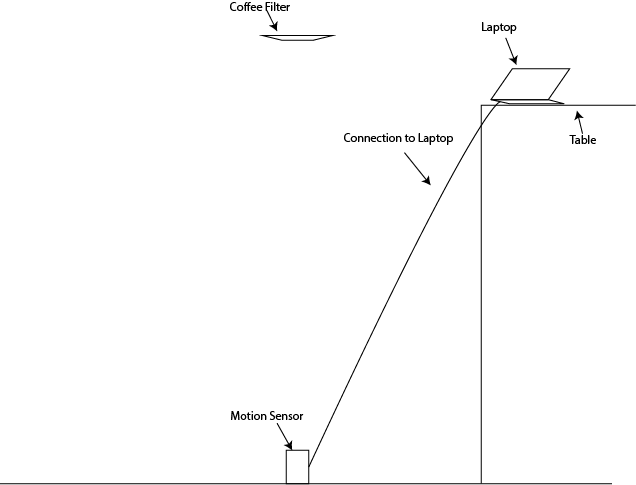
\includegraphics[width=\linewidth]{Setup.png}
    \end{figure}
    \section{Data}
    \begin{center}
        \begin{tabular}{c|>{\centering\arraybackslash}p{0.3\textwidth}>{\centering\arraybackslash}
            p{0.3\textwidth}}
            \multicolumn{3}{c}{Table 1. Mass of ten filters and filter diameter.}\\
            Trial & \(m_{10}\) (kg) & \(D\) (m)\\
            \hline
            1 & \(9.57\mathrm{x}10^{-3}\) & 0.1785\\
            2 & \(9.55\mathrm{x}10^{-3}\) & 0.1805\\
            3 & \(9.59\mathrm{x}10^{-3}\) & 0.1745\\
            4 & \(9.60\mathrm{x}10^{-3}\) & 0.1775\\
            \hline
            \(\overline{x}\) & \(9.958\mathrm{x}10^{-3}\) & 0.1777\\
            \(\sigma_x\) & \(2.2\mathrm{x}10^{-5}\) & 0.0025
        \end{tabular}\\[12pt]
        \begin{tabular}{c|>{\centering\arraybackslash}p{0.3\textwidth}>{\centering\arraybackslash}
            p{0.3\textwidth}}
            \multicolumn{3}{c}{Table 2. Dependance of terminal velocity on mass.}\\
            Trial & $m$ (kg) & $v_T$ (m/s)\\
            \hline
            1 & \(9.58\mathrm{x}10^{-4}\) & 0.752\\
            2 & \(1.916\mathrm{x}10^{-3}\) & 1.09\\
            3 & \(2.874\mathrm{x}10^{-3}\) & 1.39\\
            4 & \(3.832\mathrm{x}10^{-3}\) & 1.54\\
            5 & \(4.790\mathrm{x}10^{-3}\) & 1.76\\
        \end{tabular}
        \begin{figure}[H]
            \captionsetup{justification=centering}
            \caption{Sample plot of velocity vs time with fit to determine terminal speed.}
            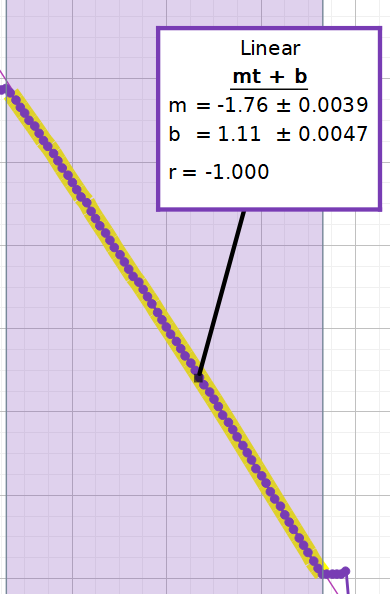
\includegraphics[height=0.7\textheight]{Figure 2.png}
        \end{figure}
        \begin{figure}[H]
            \captionsetup{justification=centering}
            \caption{Plot of \(v_T^2\) vs m with fit to find slope and error on slope.}
            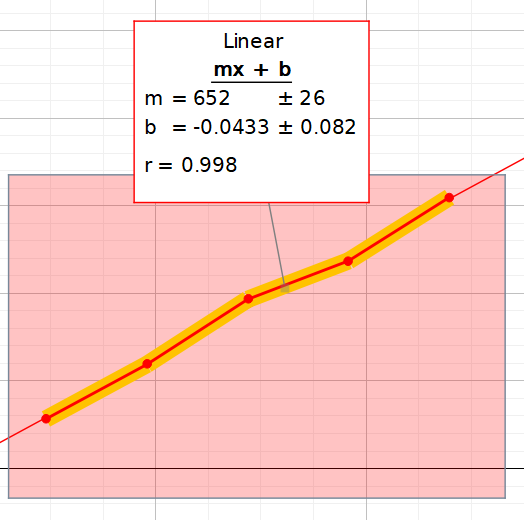
\includegraphics{Figure 3.png}
        \end{figure}
    \end{center}
    \section{Calculations}
        \begin{alignat*}{3}
            (1) ~ && F_{\mathrm{drag}} &= \frac{1}{2}C\rho Av^2\\
            &&F_g &= mg\\
            &&v &= v_T\\
            &&F_{\mathrm{drag}} &= F_g\\
            &&mg &=  \frac{1}{2}C\rho Av_T^2\\
            &&v_T^2 &= \frac{2mg}{C\rho A}\\
            &&A &= \pi r^2\\
            &&v_T^2 &= \frac{2mg}{C\rho \pi \left( \frac{D}{2} \right) ^2}\\
            &&v_T^2 &= \frac{8mg}{\pi C\rho D^2}\\
            &&S &= \frac{8g}{\pi C\rho D^2}\\
            &&C & = \frac{8mg}{\pi S\rho D^2}\\
            (2) ~ && \frac{\sigma_m}{\overline{m}} &= \frac{2.2\mathrm{x}10^{-5}~\mathrm{kg}}{9.985
            \mathrm{x}10^{-3}~\mathrm{kg}}\\
            &&& = 0.22\%\\
            &&\frac{\sigma_D}{\overline{D}} & = \frac{0.0025~\mathrm{kg}}{0.1777~\mathrm{kg}}\\
            &&& = 1.4\%\\
            &&\frac{\sigma_S}{\overline{S}} & = \frac{26~\mathrm{m}^2/\mathrm{kg}\mathrm{s}^2}{652
            ~\mathrm{m}^2/\mathrm{kg}\mathrm{s}^2}\\
            &&&=4.0\%\\
            (3) ~ && \overline{C} &= \frac{8 \cdot 9.8~\mathrm{m}/\mathrm{s}^2}{\pi \cdot 652
            ~\mathrm{m}^2/\mathrm{kg}\mathrm{s}^2 \cdot 1.2~\mathrm{kg}/\mathrm{m}^3 \cdot 
            (0.1777~\mathrm{m})^2 }\\
            &&& = 1.010\\
            (4) && C_D &= \frac{8 \cdot 9.8~\mathrm{m}/\mathrm{s}^2}{\pi \cdot 652~\mathrm{m}^2/
            \mathrm{kg}\mathrm{s}^2 \cdot 1.2~\mathrm{kg}/\mathrm{m}^3 \cdot (0.1777~\mathrm{m} + 
            0.0025)^2~\mathrm{m} }\\ 
            &&& = 0.982\\
            && C_S & = \frac{8 \cdot 9.8~\mathrm{m}/\mathrm{s}^2}{\pi \cdot (652 + 26)
            ~\mathrm{m}^2/
            \mathrm{kg}\mathrm{s}^2 \cdot 1.2~\mathrm{kg}/\mathrm{m}^3 \cdot (0.1777~\mathrm{m})^2}\\ 
            &&& = 0.971\\
            &&\sigma_C &= \sqrt{(\overline{C} - C_D)^2 + (\overline{C} - C_S)^2}\\
            &&& = \sqrt{(1.010 - 0.982)^2 + (1.010 - 0.971)^2}\\
            &&& = \sqrt{0.002275}\\
            &&& = 0.048\\
            (5) && R_e & = \frac{vD}{\nu}\\
            && \nu &= 1.516\mathrm{x}10^{-6}\\
            &&R_e &= \frac{0.75~\mathrm{m/s}\cdot0.1777~\mathrm{m}}{1.516\mathrm{x}10^{-6}~\mathrm{m}^2/\mathrm{s}}\\
            &&& = 879000
        \end{alignat*}
    \section{Conclusion}
        The error on the diameter of was greater than expected based on the precision of the meter stick. This could be caused by the variation in the diameter of the coffee filters caused by the ridges in the material. The greater than expected error could also be contributed to by slight variations in how much the coffee filter is flattened against the table by gravity. The diameter of the coffee filter when it is laying on the table may also have been different from the diameter of the filter when it is falling because the force of drag in the air may have deformed it differently than the force of gravity and normal force while it was on the table. To measure the diameter in a way that makes sure it is the same as when the coffee filter is falling we could drop it and take pictures from above and measure the diameter from the pictures.
\end{document}